\documentclass[conference]{IEEEtran}
\IEEEoverridecommandlockouts
% The preceding line is only needed to identify funding in the first footnote. If that is unneeded, please comment it out.
\usepackage{cite}
\usepackage{amsmath,amssymb,amsfonts}
\usepackage{amsmath}
\interdisplaylinepenalty=2500
\usepackage{algorithmic}
\usepackage{graphicx}
\usepackage{textcomp}
\usepackage{xcolor}
\usepackage{float}
\usepackage{booktabs}
\usepackage{mdwtab}
\usepackage{multirow}
\usepackage{tabularray}
\graphicspath{ {./figures/} }
\def\BibTeX{{\rm B\kern-.05em{\sc i\kern-.025em b}\kern-.08em
    T\kern-.1667em\lower.7ex\hbox{E}\kern-.125emX}}
    

\begin{document}

\title{Personalized phenotype encoding and prediction of pathological development from cross-sectional images.\\
% \thanks{Identify applicable funding agency here. If none, delete this.}
}
%we have more than 3 authors, so we are allowed to use the long format

\author{\IEEEauthorblockN{Connor Elkhill\IEEEauthorrefmark{1}, Ines. A Cruz-Guerrero, PhD\IEEEauthorrefmark{1}, Jiawei Liu, MS\IEEEauthorrefmark{1}, Marius George Linguraru, DPhil\IEEEauthorrefmark{2},\\Allyson Alexander, MD\IEEEauthorrefmark{4}, Brooke French, MD\IEEEauthorrefmark{5}, Antonio R. Porras, PhD\IEEEauthorrefmark{1}\IEEEauthorrefmark{6}}
\IEEEauthorblockA{\IEEEauthorrefmark{1}Department of Biostatistics and Informatics, Colorado School of Public Health, Aurora, CO}
\IEEEauthorblockA{\IEEEauthorrefmark{2}Sheikh Zayed Institute for Pediatric Surgical Innovation, Children's National Hospital, Washington, DC}
% \IEEEauthorblockA{\IEEEauthorrefmark{3}Departments of Radiology and Pediatrics,George Washington University\\School of Medicine and Health Sciences, Washington, DC}
\IEEEauthorblockA{\IEEEauthorrefmark{4}Department of Pediatric Neurosurgery, Children's Hospital Colorado, Aurora, CO}
\IEEEauthorblockA{\IEEEauthorrefmark{5}Department of Pediatric Plastic and Reconstructive Surgery, Children's Hospital Colorado, Aurora, CO}
\IEEEauthorblockA{\IEEEauthorrefmark{6}Departments of Pediatrics, Surgery and Biomedical Informatics, School of Medicine, Aurora, CO\\Email: connor.2.elkhill@cuanschutz.edu}
}


\maketitle

\begin{abstract}
The prediction of anatomical development plays a crucial role in pediatric treatment selection and planning. We present a novel deep learning architecture to make personalized predictions of pediatric normative and pathologic head development using only cross-sectional data. We designed growth predictor that learns the anatomical effects of age and sex in the presence of pathology and a novel phenotype encoder that utilizes domain adversarial training to create age- and sex-independent representations of patient phenotypes. We combined these modules to instantiate patient phenotypes to specific ages for personalized anatomical predictions conditioned to cranial pathology. We trained our models using standardized head segmentations generated from cross-sectional CT images and 3D photograms and evaluated model performance using an independent longitudinal dataset of normative subjects and children with craniosynostosis. The model achieved a head surface growth prediction error of 4.93 ± 2.29 mm and a volumetric error 0.17 ± 0.11 L in patients with cranial pathology, and 4.61 ± 3.28 mm and 0.27 ± 0.19 L for normative subjects, demonstrating state-of-the-art accuracy. Our method is the first to create age- and sex-agnostic phenotypical representations and enable personalized predictions of pathological development from only cross-sectional data.
\end{abstract}

\begin{IEEEkeywords}
predictive growth, craniosynostosis, generative adversarial network, domain adversarial training, pediatric pathological development
\end{IEEEkeywords}

\section{Introduction}
Children undergo a rapid cranial and brain growth during the first few years of life that is crucial for their cognitive development~\cite{Cao2017Developmental}. Craniosynostosis is a condition where one or more of the cranial sutures fuse prematurely and constrain cranial and brain development, often requiring surgical intervention~\cite{Mathijssen2021Updated}. However, current clinical standards to evaluate developmental anomalies rely on normative growth charts of simple metrics such as head circumference, cephalic index, or intracranial volume~\cite{Likus2014Cephalic, Meyer-Marcotty2014Three-dimensional, Rollins2010United} that cannot characterize or predict development of patients with pathology~\cite{Breakey2018Intracranial, Sgouros2005Skull, Thakkar2018Observer}.

Given the scarcity of longitudinal datasets in the pediatric population, several methods to predict cranial growth using only cross-sectional training datasets have recently been proposed. Liu et al~\cite{Liu2022Data-driven} created a normative reference of cranial growth based on age and sex using principal component analysis and temporal regression. However, this method only identified average growth trajectories in the normative pediatric population without any personalization. Porras et al~\cite{Porras2022Predictive} presented a personalized predictive model of cranial growth, but the optimization method used was not computationally feasible for large datasets. Recently, Liu et al~\cite{Liu2023Data-driven} presented a data-driven model of cranial suture growth trained only with cross-sectional data, and demonstrated state-of-the-art accuracy to predict pathologic development in patients with craniosynostosis. However, this method required the observation of the cranial sutures from computed tomography (CT) images, an image modality that requires harmful radiation exposure~\cite{Schweitzer2012Avoiding}. In a different domain, Xia et al~\cite{Xia2021Learning} utilized generative adversarial networks to learn subject-specific trajectories from a cross-sectional dataset of magnetic resonance (MR) images to predict changes in the brain morphology of patients with Alzheimer’s disease. However, their paired training scheme prevented significant anatomical temporal changes, which provided good results in adults but is not realistic in children~\cite{Hasegawa2018Developmental}.

As an alternative to CT imaging, 3D photogrammetry has become a popular radiation-free and low-cost clinical alternative to evaluate pediatric cranial malformations~\cite{Porras2019Quantification, Abdel-Alim2021Three-Dimensional}. However, it can only image the head surface and hence, prior personalized  methods~\cite{Liu2023Data-driven} relying on the identification of the cranial sutures are not feasible. We present a novel deep learning architecture designed to make personalized predictions of normative and pathologic development trained using head surface information from both cross-sectional CT images and 3D photograms, enabling radiation-free prediction of pediatric development in a clinical setting. We propose a temporal growth predictor model that learns age- and sex-specific anatomical distributions in presence or absence of pathology in the pediatric population. We also present a novel phenotype encoder that utilizes domain adversarial training to generate age- and sex-agnostic latent representations of patient phenotypes. These modules work collaboratively to generate personalized predictions of anatomical development by instantiating patient-specific phenotype representations to specific ages conditioned by the presence of pathology. The architecture was trained using only cross-sectional data from normative children and patients with craniosynostosis under the age of 10 years and was evaluated using an independent longitudinal dataset.
\section{Materials and Methods}
\subsection{Data}
After IRB approval at University of Colorado Anschutz Medical Campus (IRB \#20-1563), we collected two independent retrospective datasets: (1) a cross-sectional dataset used for model training; and (2) a longitudinal dataset used for performance evaluation. \textbf{Dataset 1} includes 2,672 cross-sectional CT images (N=2,262) and 3D photograms (N=410) of two patient populations: 2,020 normative subjects without cranial pathology (1081 male, 939 female, age $3.14 \pm 3.05$ years, range 0-10 years) and 652 patients with craniosynostosis (384 male, 268 female, age $0.64 \pm 1.04$ years, range 0-8.8 years). Dataset 2 includes two groups of longitudinal images: 61 CT image pairs from 51 normative subjects (28 male, 23 female) with average age at first image $2.24 \pm 2.22$ years and age at second image $3.55 \pm 2.71$ years (five subjects had two image pairs); and 75 pairs of 3D photograms from 75 patients with craniosynostosis (58 male, 17 female), with age of $0.61 \pm 1.07$ years at the first image and $0.85 \pm 1.18$ years at the second image.
\vspace{-1mm}
\begin{figure}[!b]
\centering
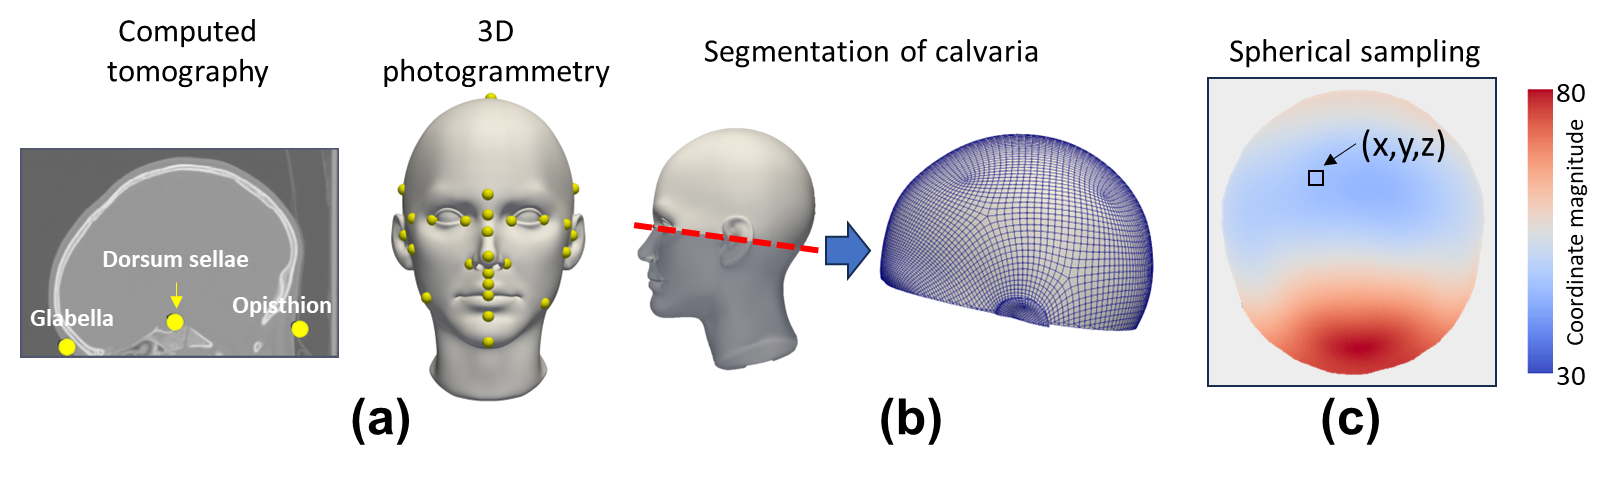
\includegraphics[width=\columnwidth]{figures/StandardizedRepresentation.png}
\caption{Standard representation of the head surface. (a) CT image or 3D photogram annotated with anatomical landmarks. Detailed annotations of landmarks for 3D photograms can be found in~\cite{Elkhill2023Geometric}. (b) Segmented head surface using the naso-tragal plane. (c) Two-dimensional standard representation of the head surface using spherical sampling, where each pixel contains the corresponding location in the head surface (X, Y, Z).}
\label{fig:standard}
\end{figure}
\subsection{Standard representation of the head surface}
We used publicly available methods to segment the head surface from CT images and 3D photograms and create standardized 2D anatomical representations~\cite{Porras2022Predictive}. In summary, adaptive thresholding~\cite{Liu2022Data-driven} and the marching cubes algorithm~\cite{Lorensen1987Marching} were used to segment the head surface from a CT image. Four cranial landmarks were automatically identified at the glabella, two temporal processes of the dorsum sellae and the opisthion in CT images. In 3D photogrammetry, we used a similar publicly available method to identify a series of anatomical landmarks on the head and face~\cite{Elkhill2023Geometric}. We used a standardized template image annotated with both sets of landmarks to align the images from both modalities given their respective landmarks. We segmented the calvaria from the rest of the head at the cranial base using the plane defined by the nasion, left and right tragion annotated on the standardized template (Fig~\ref{fig:standard}b). Finally, the head surface segmented from either image modality was sampled in spherical coordinates to create a standard 2D representation~\cite{Porras2022Predictive} Fig~\ref{fig:standard}c.
\vspace{-1mm}
\subsection{Model Architecture}
We propose a neural network architecture composed of two main modules as presented in~\ref{fig:architecture} and described below.
Personalized phenotype encoder (PPE). The goal of this module is to create a vectorized representation of the head phenotype of a patient independently from age and sex. To accomplish this, we designed a phenotype encoder that uses unsupervised representation learning and the convolutional architecture presented in~\cite{Radford2016Unsupervised} to provide a latent patient-specific phenotype representation l based on a real head shape observation \textbf{X}. Unlike previous work, we incorporate an additional phenotype discriminator (PD, purple in~\ref{fig:architecture}) and use a domain adversarial training scheme~\cite{Ganin2016Domain-Adversarial} (see details in Eq.~\ref{ppe})

to promote a phenotype representation l that is independent from age or sex. Hence, the encoder will learn to generate latent phenotype representations l that cannot be used by the PD to identify the age and sex of the patient.
Growth predictor (GP). This module uses an adversarial training scheme with the goal of generating a realistic head surface anatomy from a latent representation of a head phenotype \textbf{l} (generated by the PPE) together with information about age, sex and pathology by leveraging the learned anatomical distributions of specific patient groups in the training dataset. The GP and PPE work collaboratively to create personalized latent phenotype representations that are age- and sex-agnostic and that, when combined with specific age, sex, and pathology information, can represent the head anatomy of a specific patient. The predictor follows the convolutional architecture proposed by~\cite{Radford2016Unsupervised} but it was modified to include the conditions of patient age (encoded as a continuous variable), sex (binary encoded) and suture fusion status (one-hot encoded).
Finally, the growth discriminator (GD) (Fig~\ref{fig:architecture}, in green) enables adversarial training of both the GP and PPE. The discriminator also utilizes the convolutional architecture proposed in~\cite{Radford2016Unsupervised} to compute the Wasserstein distance~\cite{Gulrajani2017Improved} and distinguish between real head shapes and head shapes reconstructed from \textbf{l}.
\begin{figure}[!t]
\centering
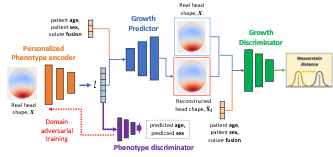
\includegraphics[width=\columnwidth]{figures/NetworkArchitecture.png}
%todo -- replace this with an SVG
\caption{Proposed neural network architecture. The personalized phenotype encoder creates a latent representation of a patient phenotype l from a real head shape that is independent of patient age or sex using domain-adversarial training. The growth predictor is trained to predict head anatomies consistent with the observed statistical distributions in the population for specific age, sex, and suture fusion status. Once trained, the phenotype representation of a patient l can be instantiated at any age using the growth predictor to produce personalized predictions.}
\label{fig:architecture}
\end{figure}
\subsection{Optimization}
We defined the prediction of age and sex from the PD as $S',A'=PD(l;\theta_{PD})$ respectively, where $\theta_{PD}$ are the learned parameters of the PD and \textbf{l} is the latent representation generated from the PPE using real input image \textbf{X}. Similar to~\cite{Wang2021Deep}, we computed the cross entropy between $S$ and $S'$ and KL divergence between the continuous distributions of $A$ and $A'$, where $A$ and $S$ are the true patient age and sex. The PPE and PD modules are trained using the following adversarial loss function:
\vspace{-2mm}
\begin{multline}\label{ppe}
    L_{PPE}=\underset{PPE}{max}\ \underset{PD}{min}\ S*log(S')\\+(1-S)*log(1-S')+A *\log\frac{A}{A'}
\end{multline}
To train the GP module, we used an adversarial scheme with the following Wasserstein loss function~\cite{Gulrajani2017Improved}.
\vspace{-2mm}
\begin{multline}\label{gp}
    L_{GP} = \mathbb{E} _{\tilde{\textbf{X}}_l \sim P_l | \textbf{X} \sim P_x} GD(\tilde{\textbf{X}}_l|A,S,C)-GD(\textbf{X}|A,S,C)\\ +\lambda _{grad} \mathbb{E} _{\hat{X}_{\sim P_{\hat{X}}}}[\| \nabla_{\hat{X}} GD(\hat{X},A,S,C,\Theta_{GD})\|_2 -1]^2, 
\end{multline}

where $P_l$ and $P_x$ are the probability distributions of the reconstructed images from the GP and $P_X$ is the probability distribution of the real input images. The second term in Eq.~\ref{gp} is the gradient penalty aimed to optimize discriminator performance and enable calculation of Wasserstein distance~\cite{Gulrajani2017Improved}. For each set of input images $\textbf{x}$ and $\tilde{\textbf{x}}$ to GD, we uniformly sampled from the distribution $P_{\hat{X}}$ random points $\hat{X}$ between the real input image distribution $P_X$ and reconstructed image distribution $P_{\hat{X}_l}$ and computed the L2-norm of the gradient with respect to the model parameters $\Theta_{GD}$. This penalty is weighted in the loss using the hyperparameter $\lambda _{grad}$.
To train our model, the two loss functions presented in Eq.~\ref{ppe} and Eq.~\ref{gp} were combined with an additional term quantifying the reconstruction error between the original image $\textbf{X}$ and the reconstructed image $\tilde{X}_l$ to promote accurate image predictions. The loss function used during training was:
\begin{multline}\label{loss}
    L = L_{GP} + \lambda_{PPE}L_{PPE}+\lambda_{rec}\left\lVert \tilde{\textbf{X}}_l-\textbf{X}\right\rVert_2
\end{multline}
\vspace*{-1mm}
where $\lambda_{PPE}$ and $\lambda_{rec}$ are hyperparameters balancing the contribution of the domain-adversarial and reconstruction losses, respectively. 
\section{Experiments and Results}
\subsection{Image preprocessing and training details}
We randomly divided Dataset 1 into training (90\%, N=1,712) and validation (10\%, N=190) sets. We processed each image as described in Section 2.2 and represented them using an image resolution of $64\times64$ pixels. To facilitate training, we normalized all image pixel components to the range [-1,1] and age to the range [0,1]. Sex was encoded as 1 for male and 0 for female and suture fusion status was one-hot encoded for each of the following sutures: sagittal, metopic, right coronal, and left coronal. Patients with lambdoid suture fusion were excluded due to insufficient data from this rare form of craniosynostosis.%todo -- maybe add a ref to lambdoid here?
Prior to model training and to facilitate convergence, the GP was first warmed up~\cite{Grigoryev2022When} for 500 epochs. Specifically, we initialized the GP and GD parameters to generate realistic anatomies using randomly sampled noise from a standard normal distribution as synthetic phenotype representations l using only the loss function from Eq.~\ref{gp}. Once initialized, we trained the entire network using Eq.~\ref{loss} and the Adam optimizer for no more than 5,000 epochs, stopping upton convergence of the validation loss or no improvements after 100 consecutive epochs. All experiments were performed on an Intel i9-10900X CPU with 32 GB RAM and an NVIDIA Quadro RTX 4000 GPU using Python 3.11 and Pytorch 2.0.1. Additional details of all hyperparameters utilized by our model, along with the trained network can be found at: [GITHUB LINK AVAILABLE UPON ACCEPTANCE]
\begin{table*}[t]
    \centering
\caption{\label{tab:results}Comparison of surface prediction and volumetric errors for patients in Dataset 2. All models were trained on Dataset 1. P-values estimated using a paired Wilcoxon signed-rank test between the proposed network and alternative methods.}
\resizebox{\textwidth}{!}{
\begin{tabular}{@{}lllll@{}}
% \begin{tblr}{columns={halign=c},rows={valign=m}, row{4-9}={mode=math},colspec={@{}lllll@{}}}
% \begin{tblr}{colspec={@{}lllll@{}}}
\toprule
Model                                            & Surface prediction Error (mm) &                                  & Volumetric Error (L)              &                                  \\ \midrule
                                                 & Craniosynostosis                                & Normative                                & Craniosynostosis                                 & Normative                                \\
Proposed network                                 & \textbf{4.93 $\pm$ 2.29}                     & 4.61 $\pm$ 3.28                     & 0.17 $\pm$ 0.11                      & 0.27 $\pm$ 0.19                     \\
Proposed network without domain-adversarial loss & 5.22 $\pm$ 2.34 (p=0.04)            & 5.22 $\pm$ 3.44 (p\textless{}0.005) & \textbf{0.16 $\pm$ 0.12} (p=0.21)             & 0.29 $\pm$ 0.21 (p=0.09)            \\
Proposed network without condition of pathology  & 6.15 $\pm$ 2.02 (p\textless{}0.005) & 6.90 $\pm$ 3.48 (p\textless{}0.005) & 0.17 $\pm$ 0.12 (p=0.35)             & 0.31 $\pm$ 0.19 (p\textless{}0.005) \\
PCA model of normative development~\cite{Liu2022Data-driven}       & 5.06 $\pm$ 4.24 (p=0.20)            & \textbf{3.77 $\pm$ 2.80} (p=0.144)           & 0.28 $\pm$ 0.24  (p\textless{}0.005) & 0.26 $\pm$ 0.20 (p=0.06)            \\
Conditional-DCGAN~\cite{Radford2016Unsupervised}                       & 5.39 $\pm$ 2.28 (p\textless{}0.005) & 5.29 $\pm$ 3.51 (p=0.01)            & 0.17 $\pm$ 0.14 (p=0.80)             & \textbf{0.22 $\pm$ 0.19} (p=0.03)            \\
Brain Ageing GAN~\cite{Xia2021Learning}                        & 6.63 $\pm$ 3.81 (p\textless{}0.005) & 7.20 $\pm$ 5.57 (p\textless{}0.005) & 0.26 $\pm$ 0.18 (p\textless{}0.005)  & 0.29 $\pm$ 0.27 (p=0.93)            \\ \bottomrule
\end{tabular}}
\end{table*}
\subsection{Performance Evaluation}
We evaluated the predictive accuracy of our model using Dataset 2. Each longitudinal image pair was organized in a bi-directional fashion resulting in 272 total pairs (122 images of normative subjects, 150 images of patients with craniosynostosis), which allowed evaluating predictions from the younger image to the older image and vice-versa. We computed the surface prediction error as the point-wise Euclidean distance in millimeters between each point in the predicted and true images and we evaluated difference in volume between the predicted and true head shape. Table~\ref{tab:results} shows a comparison between the performance of our proposed network and other methods including our own ablation studies: our proposed network without the use of domain-adversarial loss, our proposed network without the condition of pathology to make predictions, a publicly available PCA-based regression model of normative head development in the pediatric population~\cite{Liu2022Data-driven}, a conditional DCGAN~\cite{Radford2016Unsupervised}, and the model of brain aging progression available from~\cite{Xia2021Learning} trained on Dataset 1.
\section{Discussion}
We present a novel deep learning network trained using only cross-sectional data to make personalized predictions of anatomical development for patients with and without pathology. We demonstrated through evaluation presented in Table~\ref{tab:results} that our proposed network can infer anatomical development with state-of-the-art accuracy.
We found that the PCA-based regression model of normative development provides the lowest average surface prediction error in the normative subjects as compared to other methodologies, which we hypothesize is due to the substantially higher image resolution employed by this model ($500\times500$ image resolution)~\cite{Liu2022Data-driven}. Despite the lower image resolution of our method ($64\times64$ image resolution), the differences in surface prediction error are not significant.
We also found that the Conditional-DCGAN outperforms all other methodologies in volumetric error,  despite having a significantly increased surface prediction errors. This indicates that developmental patterns can be accurately learned without the use of any personalized predictions. 
Importantly, our proposed network achieved the lowest surface prediction error in patients with craniosynostosis. We improve performance using our proposed domain-adversarial loss function, suggesting it enables more accurate instantiation of patient phenotypes to various stages of development. Performance is also reduced when the condition of pathological status is removed, since pathology is an important mediator of pediatric development~\cite{Likus2014Cephalic}. Our model also achieved significantly improved surface prediction errors compared to a Conditional-DCGAN~\cite{Radford2016Unsupervised} (which only utilizes randomly sampled noise that is not personalized) and Brain Ageing GAN~\cite{Xia2021Learning} (because it assumes longitudinal anatomical changes are not significant, which is not realistic in pediatric development).
Finally, our network produces significantly lower volumetric errors for patients with craniosynostosis than the PCA-based regression normative model, due to its inability to make prediction of pathological development. Our model also produces lower volume errors compared to the Brain Ageing GAN, since it assumes limited anatomical changes between images. However, we found no significant differences between the volumetric errors produced by our proposed model and the Conditional-DCGAN, which we hypothesize is due to the shared training procedure and structure of the growth predictor found in both models. One limitation of our study is the limited sizes of our longitudinal evaluation datasets, since these datasets are rare in children.
Unlike previous works, the presented model does not make statistical assumptions about anatomical development and can consider pathologic development (i.e.,~\cite{Porras2022Predictive,Liu2022Data-driven}), and can create age- and sex-independent latent representations of patient phenotypes using domain-adversarial training to predict personalized development (i.e.,~\cite{Ganin2016Domain-Adversarial,Wang2021Deep}). This last advantage will enable the use of our network to study pediatric phenotypes associated with pathology using diverse datasets of children with different age and sex.
\section{Conclusion}
We presented a novel deep learning network using a growth predictor that learns age- and sex-specific anatomical distributions of pediatric head shape and a novel pheno-type encoding module that generates age- and sex-independent latent phenotype representations to predict personalized normative and pathologic anatomical devel-opment in children. The presented model showed state-of-the-art predictive accuracy evaluated on an independent longitudinal dataset. Our age- and sex-independent phenotype representations could be leveraged to study associations between patient phenotypes and pathology in diverse pediatric datasets.

\bibliographystyle{ieeetr}
\bibliography{ref-extracts}
\end{document}